% Options for packages loaded elsewhere
\PassOptionsToPackage{unicode}{hyperref}
\PassOptionsToPackage{hyphens}{url}
%
\documentclass[
]{article}
\usepackage{amsmath,amssymb}
\usepackage{lmodern}
\usepackage{iftex}
\ifPDFTeX
  \usepackage[T1]{fontenc}
  \usepackage[utf8]{inputenc}
  \usepackage{textcomp} % provide euro and other symbols
\else % if luatex or xetex
  \usepackage{unicode-math}
  \defaultfontfeatures{Scale=MatchLowercase}
  \defaultfontfeatures[\rmfamily]{Ligatures=TeX,Scale=1}
\fi
% Use upquote if available, for straight quotes in verbatim environments
\IfFileExists{upquote.sty}{\usepackage{upquote}}{}
\IfFileExists{microtype.sty}{% use microtype if available
  \usepackage[]{microtype}
  \UseMicrotypeSet[protrusion]{basicmath} % disable protrusion for tt fonts
}{}
\makeatletter
\@ifundefined{KOMAClassName}{% if non-KOMA class
  \IfFileExists{parskip.sty}{%
    \usepackage{parskip}
  }{% else
    \setlength{\parindent}{0pt}
    \setlength{\parskip}{6pt plus 2pt minus 1pt}}
}{% if KOMA class
  \KOMAoptions{parskip=half}}
\makeatother
\usepackage{xcolor}
\IfFileExists{xurl.sty}{\usepackage{xurl}}{} % add URL line breaks if available
\IfFileExists{bookmark.sty}{\usepackage{bookmark}}{\usepackage{hyperref}}
\hypersetup{
  pdftitle={R ile Tanımlayıcı İstatistikler ve Hipotez Testleri},
  pdfauthor={Funda İpekten},
  hidelinks,
  pdfcreator={LaTeX via pandoc}}
\urlstyle{same} % disable monospaced font for URLs
\usepackage[margin=1in]{geometry}
\usepackage{color}
\usepackage{fancyvrb}
\newcommand{\VerbBar}{|}
\newcommand{\VERB}{\Verb[commandchars=\\\{\}]}
\DefineVerbatimEnvironment{Highlighting}{Verbatim}{commandchars=\\\{\}}
% Add ',fontsize=\small' for more characters per line
\usepackage{framed}
\definecolor{shadecolor}{RGB}{248,248,248}
\newenvironment{Shaded}{\begin{snugshade}}{\end{snugshade}}
\newcommand{\AlertTok}[1]{\textcolor[rgb]{0.94,0.16,0.16}{#1}}
\newcommand{\AnnotationTok}[1]{\textcolor[rgb]{0.56,0.35,0.01}{\textbf{\textit{#1}}}}
\newcommand{\AttributeTok}[1]{\textcolor[rgb]{0.77,0.63,0.00}{#1}}
\newcommand{\BaseNTok}[1]{\textcolor[rgb]{0.00,0.00,0.81}{#1}}
\newcommand{\BuiltInTok}[1]{#1}
\newcommand{\CharTok}[1]{\textcolor[rgb]{0.31,0.60,0.02}{#1}}
\newcommand{\CommentTok}[1]{\textcolor[rgb]{0.56,0.35,0.01}{\textit{#1}}}
\newcommand{\CommentVarTok}[1]{\textcolor[rgb]{0.56,0.35,0.01}{\textbf{\textit{#1}}}}
\newcommand{\ConstantTok}[1]{\textcolor[rgb]{0.00,0.00,0.00}{#1}}
\newcommand{\ControlFlowTok}[1]{\textcolor[rgb]{0.13,0.29,0.53}{\textbf{#1}}}
\newcommand{\DataTypeTok}[1]{\textcolor[rgb]{0.13,0.29,0.53}{#1}}
\newcommand{\DecValTok}[1]{\textcolor[rgb]{0.00,0.00,0.81}{#1}}
\newcommand{\DocumentationTok}[1]{\textcolor[rgb]{0.56,0.35,0.01}{\textbf{\textit{#1}}}}
\newcommand{\ErrorTok}[1]{\textcolor[rgb]{0.64,0.00,0.00}{\textbf{#1}}}
\newcommand{\ExtensionTok}[1]{#1}
\newcommand{\FloatTok}[1]{\textcolor[rgb]{0.00,0.00,0.81}{#1}}
\newcommand{\FunctionTok}[1]{\textcolor[rgb]{0.00,0.00,0.00}{#1}}
\newcommand{\ImportTok}[1]{#1}
\newcommand{\InformationTok}[1]{\textcolor[rgb]{0.56,0.35,0.01}{\textbf{\textit{#1}}}}
\newcommand{\KeywordTok}[1]{\textcolor[rgb]{0.13,0.29,0.53}{\textbf{#1}}}
\newcommand{\NormalTok}[1]{#1}
\newcommand{\OperatorTok}[1]{\textcolor[rgb]{0.81,0.36,0.00}{\textbf{#1}}}
\newcommand{\OtherTok}[1]{\textcolor[rgb]{0.56,0.35,0.01}{#1}}
\newcommand{\PreprocessorTok}[1]{\textcolor[rgb]{0.56,0.35,0.01}{\textit{#1}}}
\newcommand{\RegionMarkerTok}[1]{#1}
\newcommand{\SpecialCharTok}[1]{\textcolor[rgb]{0.00,0.00,0.00}{#1}}
\newcommand{\SpecialStringTok}[1]{\textcolor[rgb]{0.31,0.60,0.02}{#1}}
\newcommand{\StringTok}[1]{\textcolor[rgb]{0.31,0.60,0.02}{#1}}
\newcommand{\VariableTok}[1]{\textcolor[rgb]{0.00,0.00,0.00}{#1}}
\newcommand{\VerbatimStringTok}[1]{\textcolor[rgb]{0.31,0.60,0.02}{#1}}
\newcommand{\WarningTok}[1]{\textcolor[rgb]{0.56,0.35,0.01}{\textbf{\textit{#1}}}}
\usepackage{graphicx}
\makeatletter
\def\maxwidth{\ifdim\Gin@nat@width>\linewidth\linewidth\else\Gin@nat@width\fi}
\def\maxheight{\ifdim\Gin@nat@height>\textheight\textheight\else\Gin@nat@height\fi}
\makeatother
% Scale images if necessary, so that they will not overflow the page
% margins by default, and it is still possible to overwrite the defaults
% using explicit options in \includegraphics[width, height, ...]{}
\setkeys{Gin}{width=\maxwidth,height=\maxheight,keepaspectratio}
% Set default figure placement to htbp
\makeatletter
\def\fps@figure{htbp}
\makeatother
\setlength{\emergencystretch}{3em} % prevent overfull lines
\providecommand{\tightlist}{%
  \setlength{\itemsep}{0pt}\setlength{\parskip}{0pt}}
\setcounter{secnumdepth}{-\maxdimen} % remove section numbering
\usepackage{array}
\usepackage{fancyhdr}
\pagestyle{fancy}
\fancyhead[LO,LE]{R ile Tanımlayıcı İstatistikler ve Hipotez Testleri}
\fancyfoot[CO,CE]{Copyright © 2022 Funda İpekten}
\fancyfoot[LE,RO]{\thepage}
\ifLuaTeX
  \usepackage{selnolig}  % disable illegal ligatures
\fi

\title{R ile Tanımlayıcı İstatistikler ve Hipotez Testleri}
\author{Funda İpekten}
\date{13 Mayıs 2022}

\begin{document}
\maketitle

\hypertarget{kuxfctuxfcphaneleri-ve-veriyi-uxe7aux11fux131rma}{%
\section{Kütüphaneleri ve veriyi
çağırma}\label{kuxfctuxfcphaneleri-ve-veriyi-uxe7aux11fux131rma}}

\begin{Shaded}
\begin{Highlighting}[]
\FunctionTok{library}\NormalTok{(magrittr)}
\FunctionTok{library}\NormalTok{(rstatix)}
\FunctionTok{library}\NormalTok{(ggplot2)}
\FunctionTok{library}\NormalTok{(forcats)}
\FunctionTok{library}\NormalTok{(PMCMRplus)}
\FunctionTok{library}\NormalTok{(readr) }
\FunctionTok{library}\NormalTok{(dplyr)}
\FunctionTok{library}\NormalTok{(moments)}
\end{Highlighting}
\end{Shaded}

\begin{Shaded}
\begin{Highlighting}[]
\NormalTok{tmp }\OtherTok{\textless{}{-}} \FunctionTok{read\_delim}\NormalTok{(}\AttributeTok{file =} \StringTok{"nafld.txt"}\NormalTok{, }\AttributeTok{col\_names =} \ConstantTok{TRUE}\NormalTok{)}
\FunctionTok{dim}\NormalTok{(tmp)}
\end{Highlighting}
\end{Shaded}

\begin{verbatim}
## [1] 40 30
\end{verbatim}

\begin{Shaded}
\begin{Highlighting}[]
\FunctionTok{head}\NormalTok{(tmp)}
\end{Highlighting}
\end{Shaded}

\begin{verbatim}
## # A tibble: 6 x 30
##   Gozlem_no  Grup Grup2   Yaş Cinsiyet Sigara Ağırlık   Boy   Bki Bki_grup
##       <dbl> <dbl> <dbl> <dbl>    <dbl>  <dbl>   <dbl> <dbl> <dbl>    <dbl>
## 1         1     1     1    40        2      0    93.7  1.6   36.6        1
## 2         2     1     1    33        1      0    95.5  1.84  28.2        0
## 3         3     1     1    51        2      0    65    1.49  29.3        0
## 4         4     1     1    37        1      0    84    1.66  30.5        1
## 5         5     1     2    35        2      0    84    1.6   32.8        1
## 6         6     1     2    37        1      0    98    1.7   33.9        1
## # ... with 20 more variables: Büyük_tansiyon <dbl>, Küçük_tansiyon <dbl>,
## #   İnsülin <dbl>, Glukoz <dbl>, AST <dbl>, ALT <dbl>, MPV <dbl>,
## #   miRNA197 <dbl>, miRNA146b <dbl>, miRNA10b <dbl>, miRNA181d <dbl>,
## #   Ağırlık1 <dbl>, Ağırlık3 <dbl>, Ağırlık6 <dbl>, Bki1 <dbl>, Bki3 <dbl>,
## #   Bki6 <dbl>, Tg1 <dbl>, Tg3 <dbl>, Tg6 <dbl>
\end{verbatim}

\hypertarget{deux11fiux15fkenlerin-kategorilerini-tanux131mlama}{%
\section{Değişkenlerin kategorilerini
tanımlama}\label{deux11fiux15fkenlerin-kategorilerini-tanux131mlama}}

\par\medskip

\begin{Shaded}
\begin{Highlighting}[]
\NormalTok{tmp }\OtherTok{\textless{}{-}}\NormalTok{ tmp }\SpecialCharTok{\%\textgreater{}\%}
\FunctionTok{mutate}\NormalTok{(}\AttributeTok{Grup =} \FunctionTok{factor}\NormalTok{(Grup, }\AttributeTok{levels =} \FunctionTok{c}\NormalTok{(}\DecValTok{0}\NormalTok{, }\DecValTok{1}\NormalTok{), }\AttributeTok{labels =} \FunctionTok{c}\NormalTok{(}\StringTok{"Kontrol"}\NormalTok{,}\StringTok{"Steatohepatit"}\NormalTok{)),}
       \AttributeTok{Grup2 =} \FunctionTok{factor}\NormalTok{(Grup2, }\AttributeTok{levels =} \FunctionTok{c}\NormalTok{(}\DecValTok{0}\NormalTok{, }\DecValTok{1}\NormalTok{, }\DecValTok{2}\NormalTok{), }\AttributeTok{labels =} \FunctionTok{c}\NormalTok{(}\StringTok{"Kontrol"}\NormalTok{,}\StringTok{"nafld\_id\_yok"}\NormalTok{, }\StringTok{"nafld\_id\_var"}\NormalTok{)),}
       \AttributeTok{Cinsiyet =} \FunctionTok{factor}\NormalTok{(Cinsiyet, }\AttributeTok{levels =} \FunctionTok{c}\NormalTok{(}\DecValTok{1}\NormalTok{, }\DecValTok{2}\NormalTok{), }\AttributeTok{labels =} \FunctionTok{c}\NormalTok{(}\StringTok{"Erkek"}\NormalTok{, }\StringTok{"Kadın"}\NormalTok{)), }
       \AttributeTok{Sigara =} \FunctionTok{factor}\NormalTok{(Sigara, }\AttributeTok{levels =} \FunctionTok{c}\NormalTok{(}\DecValTok{0}\NormalTok{, }\DecValTok{1}\NormalTok{), }\AttributeTok{labels =} \FunctionTok{c}\NormalTok{(}\StringTok{"Kullanmayan"}\NormalTok{, }\StringTok{"Kullanan"}\NormalTok{)),}
       \AttributeTok{Bki\_grup =} \FunctionTok{factor}\NormalTok{(Bki\_grup, }\AttributeTok{levels =} \FunctionTok{c}\NormalTok{(}\DecValTok{0}\NormalTok{, }\DecValTok{1}\NormalTok{)),}
       \AttributeTok{Bki1 =} \FunctionTok{factor}\NormalTok{(Bki1, }\AttributeTok{levels =} \FunctionTok{c}\NormalTok{(}\DecValTok{0}\NormalTok{, }\DecValTok{1}\NormalTok{), }\AttributeTok{labels =} \FunctionTok{c}\NormalTok{(}\StringTok{"Obez olmayan"}\NormalTok{, }\StringTok{"Obez olan"}\NormalTok{)),}
       \AttributeTok{Bki3 =} \FunctionTok{factor}\NormalTok{(Bki3, }\AttributeTok{levels =} \FunctionTok{c}\NormalTok{(}\DecValTok{0}\NormalTok{, }\DecValTok{1}\NormalTok{), }\AttributeTok{labels =} \FunctionTok{c}\NormalTok{(}\StringTok{"Obez olmayan"}\NormalTok{, }\StringTok{"Obez olan"}\NormalTok{)),}
       \AttributeTok{Bki6 =} \FunctionTok{factor}\NormalTok{(Bki6, }\AttributeTok{levels =} \FunctionTok{c}\NormalTok{(}\DecValTok{0}\NormalTok{, }\DecValTok{1}\NormalTok{), }\AttributeTok{labels =} \FunctionTok{c}\NormalTok{(}\StringTok{"Obez olmayan"}\NormalTok{, }\StringTok{"Obez olan"}\NormalTok{)))}
\end{Highlighting}
\end{Shaded}

\begin{Shaded}
\begin{Highlighting}[]
\FunctionTok{dim}\NormalTok{(tmp)}
\end{Highlighting}
\end{Shaded}

\begin{verbatim}
## [1] 40 30
\end{verbatim}

\begin{Shaded}
\begin{Highlighting}[]
\FunctionTok{head}\NormalTok{(tmp)}
\end{Highlighting}
\end{Shaded}

\begin{verbatim}
## # A tibble: 6 x 30
##   Gozlem_no Grup        Grup2   Yaş Cinsiyet Sigara Ağırlık   Boy   Bki Bki_grup
##       <dbl> <fct>       <fct> <dbl> <fct>    <fct>    <dbl> <dbl> <dbl> <fct>   
## 1         1 Steatohepa~ nafl~    40 Kadın    Kulla~    93.7  1.6   36.6 1       
## 2         2 Steatohepa~ nafl~    33 Erkek    Kulla~    95.5  1.84  28.2 0       
## 3         3 Steatohepa~ nafl~    51 Kadın    Kulla~    65    1.49  29.3 0       
## 4         4 Steatohepa~ nafl~    37 Erkek    Kulla~    84    1.66  30.5 1       
## 5         5 Steatohepa~ nafl~    35 Kadın    Kulla~    84    1.6   32.8 1       
## 6         6 Steatohepa~ nafl~    37 Erkek    Kulla~    98    1.7   33.9 1       
## # ... with 20 more variables: Büyük_tansiyon <dbl>, Küçük_tansiyon <dbl>,
## #   İnsülin <dbl>, Glukoz <dbl>, AST <dbl>, ALT <dbl>, MPV <dbl>,
## #   miRNA197 <dbl>, miRNA146b <dbl>, miRNA10b <dbl>, miRNA181d <dbl>,
## #   Ağırlık1 <dbl>, Ağırlık3 <dbl>, Ağırlık6 <dbl>, Bki1 <fct>, Bki3 <fct>,
## #   Bki6 <fct>, Tg1 <dbl>, Tg3 <dbl>, Tg6 <dbl>
\end{verbatim}

\par\medskip

\hypertarget{tanux131mlayux131cux131-istatistikler}{%
\section{Tanımlayıcı
İstatistikler}\label{tanux131mlayux131cux131-istatistikler}}

Dağılımlar,

\begin{itemize}
\tightlist
\item
  Yer (Location) ölçüleri (Aritmetik ortalama, medyan, mod, kantiller,
  \ldots)
\item
  Yaygınlık (Spread) ölçüleri (Varyans, standart sapma, kantiller arası
  uzaklık, \ldots)
\item
  Şekil (Shape) Ölçüleri (Çarpıklık, Basıklık)
\end{itemize}

olmak üzere 3 farklı ölçüm ile temsil edilirler. Bu ölçüler tanımlayıcı
istatistikler olarak adlandırılır.

\begin{Shaded}
\begin{Highlighting}[]
\CommentTok{\# Nicel değişken için tanımlayıcı istatistikler (AST)}

\NormalTok{descAST }\OtherTok{\textless{}{-}}\NormalTok{ tmp }\SpecialCharTok{\%\textgreater{}\%}
  \FunctionTok{group\_by}\NormalTok{(Grup) }\SpecialCharTok{\%\textgreater{}\%}
  \FunctionTok{summarise}\NormalTok{(}\AttributeTok{N =} \FunctionTok{n}\NormalTok{(), }\AttributeTok{Ortalama =} \FunctionTok{mean}\NormalTok{(AST), }\AttributeTok{Standart.sapma =} \FunctionTok{round}\NormalTok{(}\FunctionTok{sd}\NormalTok{(AST), }\DecValTok{2}\NormalTok{), }\AttributeTok{Medyan =} \FunctionTok{median}\NormalTok{(AST),}
            \AttributeTok{Q1 =} \FunctionTok{quantile}\NormalTok{(AST, .}\DecValTok{25}\NormalTok{), }\AttributeTok{Q3 =} \FunctionTok{quantile}\NormalTok{(AST, .}\DecValTok{75}\NormalTok{), }
\NormalTok{            Çarpıklık }\OtherTok{=} \FunctionTok{round}\NormalTok{(}\FunctionTok{skewness}\NormalTok{(AST),}\DecValTok{2}\NormalTok{), Basıklık }\OtherTok{=} \FunctionTok{round}\NormalTok{(}\FunctionTok{kurtosis}\NormalTok{(AST),}\DecValTok{2}\NormalTok{))}
\FunctionTok{print.data.frame}\NormalTok{(descAST)}
\end{Highlighting}
\end{Shaded}

\begin{verbatim}
##            Grup  N Ortalama Standart.sapma Medyan    Q1   Q3 Çarpıklık Basıklık
## 1       Kontrol 20    22.50           5.20     21 18.00 26.5      0.34     1.97
## 2 Steatohepatit 20    50.45          20.21     45 34.75 59.0      1.18     3.56
\end{verbatim}

\par\medskip

\begin{Shaded}
\begin{Highlighting}[]
\NormalTok{tmp }\SpecialCharTok{\%\textgreater{}\%}
  \FunctionTok{ggplot}\NormalTok{(}\FunctionTok{aes}\NormalTok{(}\AttributeTok{x =} \FunctionTok{factor}\NormalTok{(Grup), }\AttributeTok{y =}\NormalTok{ AST)) }\SpecialCharTok{+} 
    \FunctionTok{geom\_boxplot}\NormalTok{(}\AttributeTok{fill =} \StringTok{"gray90"}\NormalTok{) }\SpecialCharTok{+}
    \FunctionTok{theme\_bw}\NormalTok{(}\AttributeTok{base\_size =} \DecValTok{14}\NormalTok{)}\SpecialCharTok{+}
  \FunctionTok{labs}\NormalTok{(}\AttributeTok{x=}\StringTok{"Grup"}\NormalTok{, }\AttributeTok{y=}\StringTok{"AST"}\NormalTok{)}
\end{Highlighting}
\end{Shaded}

\includegraphics{Fundaİpekten_Rmarkdown_files/figure-latex/boxplot-AST-1.pdf}

\par\medskip

\begin{Shaded}
\begin{Highlighting}[]
\CommentTok{\# Nitel değişken için tanımlayıcı istatistikler ( Bki\_grup)}

\NormalTok{tmp }\SpecialCharTok{\%\textgreater{}\%}
  \FunctionTok{group\_by}\NormalTok{(Grup2) }\SpecialCharTok{\%\textgreater{}\%}
  \FunctionTok{summarise}\NormalTok{(}\AttributeTok{N =} \FunctionTok{n}\NormalTok{(), }\AttributeTok{n\_obez =} \FunctionTok{sum}\NormalTok{(Bki\_grup }\SpecialCharTok{==} \DecValTok{1}\NormalTok{),    }\CommentTok{\# 1: Obez olan}
            \AttributeTok{Percentage =} \FunctionTok{round}\NormalTok{(}\DecValTok{100} \SpecialCharTok{*}\NormalTok{ n\_obez }\SpecialCharTok{/}\NormalTok{ N, }\DecValTok{2}\NormalTok{)) }\SpecialCharTok{\%\textgreater{}\%}
\NormalTok{print.data.frame}
\end{Highlighting}
\end{Shaded}

\begin{verbatim}
##          Grup2  N n_obez Percentage
## 1      Kontrol 20      5         25
## 2 nafld_id_yok  8      2         25
## 3 nafld_id_var 12     12        100
\end{verbatim}

\par\medskip

\begin{Shaded}
\begin{Highlighting}[]
\CommentTok{\# Grouped/Stacked bar graphs.}
\NormalTok{tmp }\SpecialCharTok{\%\textgreater{}\%}
  \FunctionTok{mutate}\NormalTok{(}\AttributeTok{Grup2 =} \FunctionTok{factor}\NormalTok{(Grup2), }\AttributeTok{Bki\_grup =} \FunctionTok{factor}\NormalTok{(Bki\_grup)) }\SpecialCharTok{\%\textgreater{}\%}
  \FunctionTok{group\_by}\NormalTok{(Grup2, Bki\_grup) }\SpecialCharTok{\%\textgreater{}\%}
  \FunctionTok{summarise}\NormalTok{(}\AttributeTok{N =} \FunctionTok{n}\NormalTok{()) }\SpecialCharTok{\%\textgreater{}\%}
  \FunctionTok{group\_by}\NormalTok{(Grup2, }\AttributeTok{.drop =} \ConstantTok{TRUE}\NormalTok{) }\SpecialCharTok{\%\textgreater{}\%}
  \FunctionTok{mutate}\NormalTok{(}\AttributeTok{Percentage =} \DecValTok{100} \SpecialCharTok{*}\NormalTok{ N }\SpecialCharTok{/} \FunctionTok{sum}\NormalTok{(N)) }\SpecialCharTok{\%\textgreater{}\%}
  \FunctionTok{ggplot}\NormalTok{(}\FunctionTok{aes}\NormalTok{(}\AttributeTok{x =}\NormalTok{ Grup2, }\AttributeTok{y =}\NormalTok{ Percentage, }\AttributeTok{fill =}\NormalTok{ Bki\_grup)) }\SpecialCharTok{+} 
    \FunctionTok{geom\_bar}\NormalTok{(}\AttributeTok{stat =} \StringTok{"identity"}\NormalTok{, }\AttributeTok{colour =} \StringTok{"white"}\NormalTok{, }
             \AttributeTok{position =} \FunctionTok{position\_dodge}\NormalTok{(), }\AttributeTok{width =}\NormalTok{ .}\DecValTok{7}\NormalTok{) }\SpecialCharTok{+}
    \FunctionTok{theme\_bw}\NormalTok{(}\AttributeTok{base\_size =} \DecValTok{14}\NormalTok{) }\SpecialCharTok{+} 
    \FunctionTok{theme}\NormalTok{(}\AttributeTok{panel.background =} \FunctionTok{element\_rect}\NormalTok{(}\AttributeTok{fill =} \StringTok{"gray95"}\NormalTok{)) }\SpecialCharTok{+}
    \FunctionTok{labs}\NormalTok{(}\AttributeTok{x =} \StringTok{"Grup 2"}\NormalTok{) }\SpecialCharTok{+} 
    \FunctionTok{scale\_fill\_discrete}\NormalTok{(}\AttributeTok{name =} \StringTok{"Bki Grup"}\NormalTok{, }
                        \AttributeTok{labels =} \FunctionTok{c}\NormalTok{(}\StringTok{"Obez olan"}\NormalTok{, }\StringTok{"Obez olmayan"}\NormalTok{))}
\end{Highlighting}
\end{Shaded}

\includegraphics{Fundaİpekten_Rmarkdown_files/figure-latex/Grouped/Stacked bar graphs-1.pdf}

\begin{Shaded}
\begin{Highlighting}[]
\CommentTok{\# Grouped/Stacked bar graphs.}
\NormalTok{myplot }\OtherTok{\textless{}{-}}\NormalTok{ tmp }\SpecialCharTok{\%\textgreater{}\%}
  \FunctionTok{mutate}\NormalTok{(}\AttributeTok{Grup2 =} \FunctionTok{factor}\NormalTok{(Grup2), }\AttributeTok{Bki\_grup =} \FunctionTok{factor}\NormalTok{(Bki\_grup)) }\SpecialCharTok{\%\textgreater{}\%}
  \FunctionTok{group\_by}\NormalTok{(Grup2, Bki\_grup) }\SpecialCharTok{\%\textgreater{}\%}
  \FunctionTok{summarise}\NormalTok{(}\AttributeTok{N =} \FunctionTok{n}\NormalTok{()) }\SpecialCharTok{\%\textgreater{}\%}
  \FunctionTok{group\_by}\NormalTok{(Grup2, }\AttributeTok{.drop =} \ConstantTok{TRUE}\NormalTok{) }\SpecialCharTok{\%\textgreater{}\%}
  \FunctionTok{mutate}\NormalTok{(}\AttributeTok{Percentage =} \DecValTok{100} \SpecialCharTok{*}\NormalTok{ N }\SpecialCharTok{/} \FunctionTok{sum}\NormalTok{(N)) }\SpecialCharTok{\%\textgreater{}\%}
  \FunctionTok{ggplot}\NormalTok{(}\FunctionTok{aes}\NormalTok{(}\AttributeTok{x =}\NormalTok{ Grup2, }\AttributeTok{y =}\NormalTok{ Percentage, }\AttributeTok{fill =}\NormalTok{ Bki\_grup)) }\SpecialCharTok{+} 
    \FunctionTok{geom\_bar}\NormalTok{(}\AttributeTok{stat =} \StringTok{"identity"}\NormalTok{, }\AttributeTok{colour =} \StringTok{"white"}\NormalTok{, }\AttributeTok{width =}\NormalTok{ .}\DecValTok{7}\NormalTok{) }\SpecialCharTok{+}
    \FunctionTok{theme\_bw}\NormalTok{(}\AttributeTok{base\_size =} \DecValTok{14}\NormalTok{) }\SpecialCharTok{+} 
    \FunctionTok{theme}\NormalTok{(}\AttributeTok{panel.background =} \FunctionTok{element\_rect}\NormalTok{(}\AttributeTok{fill =} \StringTok{"gray95"}\NormalTok{)) }\SpecialCharTok{+} 
    \FunctionTok{scale\_fill\_discrete}\NormalTok{(}\AttributeTok{name =} \StringTok{"Bki Grup"}\NormalTok{, }
                        \AttributeTok{labels =} \FunctionTok{c}\NormalTok{(}\StringTok{"Obez olan"}\NormalTok{, }\StringTok{"Obez olmayan"}\NormalTok{))}
\FunctionTok{print}\NormalTok{(myplot)}
\end{Highlighting}
\end{Shaded}

\includegraphics{Fundaİpekten_Rmarkdown_files/figure-latex/Grouped/Stacked bar graphs-2.pdf}

\begin{Shaded}
\begin{Highlighting}[]
\NormalTok{myplot }\SpecialCharTok{+} 
  \FunctionTok{geom\_label}\NormalTok{(}\FunctionTok{aes}\NormalTok{(}\AttributeTok{label =} \FunctionTok{paste0}\NormalTok{(}\FunctionTok{round}\NormalTok{(Percentage, }\DecValTok{2}\NormalTok{), }\StringTok{"\%"}\NormalTok{), }\AttributeTok{colour =}\NormalTok{ Bki\_grup), }
             \AttributeTok{size =} \DecValTok{4}\NormalTok{, }\AttributeTok{fontface =} \StringTok{"bold"}\NormalTok{, }\AttributeTok{fill =} \StringTok{"white"}\NormalTok{, }\AttributeTok{show.legend =} \ConstantTok{FALSE}\NormalTok{,}
             \AttributeTok{label.padding =} \FunctionTok{unit}\NormalTok{(}\FloatTok{0.35}\NormalTok{, }\StringTok{"lines"}\NormalTok{), }
             \AttributeTok{position =} \FunctionTok{position\_stack}\NormalTok{(}\AttributeTok{vjust =}\NormalTok{ .}\DecValTok{50}\NormalTok{))}
\end{Highlighting}
\end{Shaded}

\includegraphics{Fundaİpekten_Rmarkdown_files/figure-latex/Grouped/Stacked bar graphs-3.pdf}

\hypertarget{normallik-testleri}{%
\section{Normallik Testleri}\label{normallik-testleri}}

İstatistiksel analizler çeşitli varsayımlara dayanmaktadır. Bu
varsayımlardan bir tanesi de değişkenlerin normal dağılıma sahip olması
varsayımıdır.

Çoğu zaman bu varsayım ihmal edilerek güvenilir olmayan sonuçlar ortaya
çıkmaktadır.

İstatistiksel yöntemlerin birçoğunda yapılacak analizin türüne bağlı
olarak veriler normal dağılıma sahip olmak zorundadır.

Ancak bu varsayımın her zaman sağlanamadığı ve çeşitli sebeplerle zaman
zaman verilerin dağılımında normalden sapmaların ortaya çıktığı
görülmektedir.

Dağılımın normal olup olmadığı üç farklı yaklaşımdan hareketle ortaya
konulabilir. Bu yaklaşımlar;

\begin{itemize}
\tightlist
\item
  Çarpıklık (\(\alpha_3\)) ve basıklık (\(\alpha_4\)) ölçüleri
\item
  Grafikler (Histogram, Q-Q, P-P, \ldots)
\item
  Hipotez testleri (Shapiro-Wilk, Kolmogorov-Smirnov, Anderson-Darling,
  \ldots)
\end{itemize}

\textbf{\url{http://biosoft.erciyes.edu.tr/app/MVN}}

\begin{Shaded}
\begin{Highlighting}[]
\CommentTok{\# Ağırlığa ait çarpıklık ve basıklık ölçüleri}

\NormalTok{sekil\_olcusu }\OtherTok{\textless{}{-}}\NormalTok{ tmp }\SpecialCharTok{\%\textgreater{}\%}
  \FunctionTok{group\_by}\NormalTok{(Grup) }\SpecialCharTok{\%\textgreater{}\%}
  \FunctionTok{summarise}\NormalTok{(}\AttributeTok{N =} \FunctionTok{n}\NormalTok{(), Çarpıklık }\OtherTok{=} \FunctionTok{round}\NormalTok{(}\FunctionTok{skewness}\NormalTok{(Ağırlık),}\DecValTok{2}\NormalTok{), }
\NormalTok{                     Basıklık }\OtherTok{=} \FunctionTok{round}\NormalTok{(}\FunctionTok{kurtosis}\NormalTok{(Ağırlık),}\DecValTok{2}\NormalTok{))}
\FunctionTok{print.data.frame}\NormalTok{(sekil\_olcusu)}
\end{Highlighting}
\end{Shaded}

\begin{verbatim}
##            Grup  N Çarpıklık Basıklık
## 1       Kontrol 20      0.63     3.51
## 2 Steatohepatit 20     -0.15     2.97
\end{verbatim}

\begin{Shaded}
\begin{Highlighting}[]
\CommentTok{\# Ağırlığa ait histogram grafiği}

\NormalTok{tmp }\SpecialCharTok{\%\textgreater{}\%}
\FunctionTok{filter}\NormalTok{(Bki\_grup}\SpecialCharTok{==}\DecValTok{1}\NormalTok{)}\SpecialCharTok{\%\textgreater{}\%}     \CommentTok{\# 1: Obez olan}
\FunctionTok{ggplot}\NormalTok{(}\FunctionTok{aes}\NormalTok{(}\AttributeTok{x =}\NormalTok{ Ağırlık, }\AttributeTok{y=}\NormalTok{ ..density..))}\SpecialCharTok{+}
  \FunctionTok{geom\_histogram}\NormalTok{(}\AttributeTok{bins =} \DecValTok{12}\NormalTok{, }\AttributeTok{fill =} \StringTok{"gray90"}\NormalTok{, }\AttributeTok{colour =} \StringTok{"gray60"}\NormalTok{)}\SpecialCharTok{+}
  \FunctionTok{geom\_density}\NormalTok{(}\AttributeTok{colour =} \StringTok{"blue"}\NormalTok{, }\AttributeTok{linewidth =} \DecValTok{2}\NormalTok{)}\SpecialCharTok{+}
  \FunctionTok{theme\_bw}\NormalTok{(}\AttributeTok{base\_size =} \DecValTok{14}\NormalTok{) }\SpecialCharTok{+} 
    \FunctionTok{labs}\NormalTok{(}\AttributeTok{y =}\StringTok{"Yoğunluk"}\NormalTok{, }\AttributeTok{x =} \FunctionTok{expression}\NormalTok{(}\StringTok{"Ağırlık"}\NormalTok{))}
\end{Highlighting}
\end{Shaded}

\includegraphics{Fundaİpekten_Rmarkdown_files/figure-latex/Ağırlığa ait histogram grafiği-1.pdf}

\begin{Shaded}
\begin{Highlighting}[]
\CommentTok{\# Ağırlığa ait Q{-}Q grafiği}

\FunctionTok{qqnorm}\NormalTok{(tmp }\SpecialCharTok{\%$\%}\NormalTok{ Ağırlık, }\AttributeTok{pch =} \DecValTok{1}\NormalTok{, }\AttributeTok{frame =}\NormalTok{ T)}
\FunctionTok{qqline}\NormalTok{(tmp }\SpecialCharTok{\%$\%}\NormalTok{ Ağırlık, }\AttributeTok{col =} \StringTok{"steelblue"}\NormalTok{, }\AttributeTok{lwd =} \DecValTok{2}\NormalTok{)}
\end{Highlighting}
\end{Shaded}

\includegraphics{Fundaİpekten_Rmarkdown_files/figure-latex/Ağırlığa ait Q-Q grafiği-1.pdf}

\begin{Shaded}
\begin{Highlighting}[]
\CommentTok{\# Ağırlığa ait Shapiro{-}Wilk hipotez testi}

\CommentTok{\# H0: Normal dağılıma uygunluk vardır. }
\CommentTok{\# (Serinin dağılımı ile normal dağılım arasında istatistiksel bakımdan anlamlı bir fark yoktur.)}

\CommentTok{\# H1: Normal dağılıma uygunluk yoktur. }
\CommentTok{\# (Serinin dağılımı ile normal dağılım arasında istatistiksel bakımdan anlamlı bir fark vardır.)}

\NormalTok{tmp }\SpecialCharTok{\%\textgreater{}\%}
  \FunctionTok{filter}\NormalTok{(Bki\_grup }\SpecialCharTok{==} \DecValTok{1}\NormalTok{) }\SpecialCharTok{\%$\%}    \CommentTok{\# 1: Obez olan}
  \FunctionTok{shapiro.test}\NormalTok{(Ağırlık)}
\end{Highlighting}
\end{Shaded}

\begin{verbatim}
## 
##  Shapiro-Wilk normality test
## 
## data:  Ağırlık
## W = 0.96649, p-value = 0.7047
\end{verbatim}

\hypertarget{hipotez-testleri}{%
\section{Hipotez Testleri}\label{hipotez-testleri}}

\textbf{Hipotez:} Doğruluğu bir araştırma ya da deney ile test edilmeye
çalışılan öngörülere, iddialara, hükümlere denir.

\textbf{Hipotez testleri:} Elde edilen değerlerin ya da varılan
sonuçların istatistiksel olarak anlamlı olup olmadığını (önem taşıyıp
taşımadığını) test etmek için başvurulan yöntemdir. Hipotez testlerinde
birbirinin zıddı hükümler içeren iki hipotez bulunmaktadır.

\textbf{Sıfır Hipotezi (Yokluk Hipotezi):}Benzerlik, eşitlik,
bağımsızlık, ilişkisizlik gibi ifadeler kullanılmaktadır. \(H_0\)
sembolü ile gösterilmektedir. Örneklemden elde edilen sonuçların
tesadüfe bağlı olduğunu ifade etmektedir.

\begin{itemize}
\tightlist
\item
  \(H_0\):İdrar yolu enfeksiyonu olan ve olmayan gebelerin CRP düzeyleri
  birbirine eşittir.
\end{itemize}

\textbf{Karşıt Hipotez (Alternatif Hipotez):}Farklılığı, eşit olmayan
durumu, bağımlılık gibi ifadeler kullanılmaktadır. \(H_1\) sembolü ile
gösterilmektedir. Örneklemden elde edilen sonuçların tesadüfe bağlı
olmadığını ifade etmektedir.

\begin{itemize}
\tightlist
\item
  \(H_1\):İdrar yolu enfeksiyonu olan ve olmayan gebelerin CRP düzeyleri
  birbirine eşit değildir.
\end{itemize}

Hipotez testleri sonucunda \(H_0\) hipotezi \textbf{kabul} veya
\textbf{red} edilir.

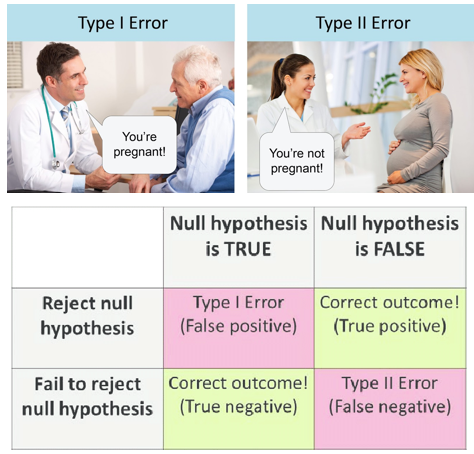
\includegraphics[width=0.5\linewidth,height=0.5\textheight]{picture_type}

\textbf{İstatistiksel Karar}

Tüm testlerin sonunda, \(H_0\) hipotezinin reddedilmesi halinde
düşülecek gerçek hata miktarı(p değeri) belirlenir. Bu değer önceden
belirlenmiş olan \(\alpha\) değeri ile karşılaştırılır.

\begin{itemize}
\item
  \(p\) \textless{} \(\alpha\) ise \(H_0\) hipotezi reddedilir. Bu
  karar, örneklemden elde edilen sonuçların istatistiksel açıdan önemli
  olduğu yani \(H_1\) hipotezinin kabul edildiği anlamına gelir.
\item
  \(p\) \textgreater{} \(\alpha\) ise \(H_0\) hipotezi kabul edilir. Bu
  karar, örneklemden elde edilen sonuçların istatistiksel açıdan önemli
  olmadığı anlamına gelir.
\end{itemize}

\textbf{İstatistiksel Önemlilik Testinin Seçim Kriterleri}

\begin{itemize}
\tightlist
\item
  Kurulan hipotezde parametre kullanılıp kullanılmamasına,
\item
  Parametre sayısına,
\item
  Örnek(grup) sayısına,
\item
  Örneklemin bağımlı olup olmadığına,
\item
  Test edilecek değişken sayısına bağlı olarak farklı biçimlerde
  sınıflandırılır.
\end{itemize}

\textbf{Test edilen değişken sayısına göre}

\begin{itemize}
\tightlist
\item
  Tek değişkenli önemlilik testleri
\item
  Çok değişkenli önemlilik testleri
\end{itemize}

\textbf{Kurulan hipotezin parametreye dayalı olup olmadığına göre}

\begin{itemize}
\tightlist
\item
  Parametrik önemlilik testleri
\item
  Parametrik olmayan önemlilik testleri
\end{itemize}

\textbf{Örneklem sayısına göre}

\begin{itemize}
\tightlist
\item
  Tek örneklem testleri
\item
  İki örneklem testleri
\item
  k-örneklem testlerii
\end{itemize}

\textbf{Örneklemin bağımlı olup olmadığına göre}

\begin{enumerate}
\def\labelenumi{\arabic{enumi}.}
\tightlist
\item
  \textbf{Bağımlı örneklem testleri}
\end{enumerate}

\begin{itemize}
\tightlist
\item
  Bağımlı iki örneklem testleri
\item
  Bağımlı k-örneklem testleri
\end{itemize}

\begin{enumerate}
\def\labelenumi{\arabic{enumi}.}
\setcounter{enumi}{1}
\tightlist
\item
  \textbf{Bağımsız örneklem testleri}
\end{enumerate}

\begin{itemize}
\tightlist
\item
  Bağımsız iki örneklem testleri
\item
  Bağımsız k-örneklem testleri
\end{itemize}

\textbf{Hipotezin kuruluş biçimine göre}

\begin{itemize}
\tightlist
\item
  Ortalamaya dayalı testler
\item
  Orana dayalı testler
\item
  Gözlem sayılarına dayalı testler
\item
  Dağılıma dayalı testler
\item
  Sıralama puanlarına dayalı testler
\item
  Uyuma, uygunluğa dayalı testler
\item
  \ldots{}
\end{itemize}

\hypertarget{tek-uxf6rneklem-t-testi-one-sample-t-test}{%
\subsection{Tek örneklem t testi (One sample t
test)}\label{tek-uxf6rneklem-t-testi-one-sample-t-test}}

\textbf{Varsayımlar}

\begin{itemize}
\tightlist
\item
  Örneklem ilgili kitleden \textbf{rastgele} ve \textbf{tek örneklem}
  grubundan seçilmiş olmalıdır.
\item
  İlgili değişken nicel olmalıdır.
\item
  ilgili değişken normal dağılıma uymalıdır.
\item
  Kitle ortalamasının belli bir değere eşit olup olmadığı test edilir.
\end{itemize}

\textbf{Örnek:} Obez olan grupta ALT düzeyinin ortalamasının 35'e eşit
olup olmadığı araştırılmak istenmektedir. İlgili örnek için hipotez
aşağıdaki gibidir.

\begin{align*}
  H_0:&~ \mu_{ALT} = 35 \\
  H_1:&~ \mu_{ALT} \neq 35
\end{align*}

\begin{Shaded}
\begin{Highlighting}[]
\CommentTok{\# Tek örneklem t testi}

\NormalTok{tmp }\SpecialCharTok{\%\textgreater{}\%}
  \FunctionTok{filter}\NormalTok{(Bki\_grup }\SpecialCharTok{==} \DecValTok{1}\NormalTok{) }\SpecialCharTok{\%$\%}   \CommentTok{\# 1: Obez olan}
  \FunctionTok{t.test}\NormalTok{(}\AttributeTok{x =}\NormalTok{ ALT, }\AttributeTok{alternative =} \StringTok{"two.sided"}\NormalTok{, }\AttributeTok{mu =} \DecValTok{35}\NormalTok{, }\AttributeTok{conf.level =}\NormalTok{ .}\DecValTok{95}\NormalTok{)}
\end{Highlighting}
\end{Shaded}

\begin{verbatim}
## 
##  One Sample t-test
## 
## data:  ALT
## t = 3.144, df = 18, p-value = 0.005612
## alternative hypothesis: true mean is not equal to 35
## 95 percent confidence interval:
##  43.87027 79.60342
## sample estimates:
## mean of x 
##  61.73684
\end{verbatim}

\hypertarget{iux15faret-testi-sign-test}{%
\subsection{İşaret testi (Sign test)}\label{iux15faret-testi-sign-test}}

\textbf{Varsayımlar}

\begin{itemize}
\tightlist
\item
  Örneklem ilgili kitleden \textbf{rastgele} ve \textbf{tek örneklem
  grubundan} seçilmiş olmalıdır.
\item
  İlgili değişken \textbf{nicel} olmalıdır.
\item
  ilgili değişken normal dağılıma uymamalıdır.
\item
  Kitle ortalamasının belli bir değere eşit olup olmadığı test edilir.
\end{itemize}

\textbf{Örnek:} Obez olan grupta Tg1 düzeyinin ortancasının 150'ye eşit
olup olmadığı araştırılmak istenmektedir. İlgili örnek için hipotez
aşağıdaki gibidir.

\begin{align*}
  H_0:&~ \mu_{Tg1} = 150 \\
  H_1:&~ \mu_{Tg1} \neq 150
  
\end{align*}

\begin{Shaded}
\begin{Highlighting}[]
\CommentTok{\# İşaret testi}

\NormalTok{tmp }\SpecialCharTok{\%\textgreater{}\%}
  \FunctionTok{filter}\NormalTok{( Bki\_grup }\SpecialCharTok{==} \DecValTok{1}\NormalTok{) }\SpecialCharTok{\%$\%}   \CommentTok{\# 1: Obez olan}
  \FunctionTok{wilcox.test}\NormalTok{(}\AttributeTok{x =}\NormalTok{ Tg1, }\AttributeTok{alternative =} \StringTok{"two.sided"}\NormalTok{, }\AttributeTok{mu =} \DecValTok{150}\NormalTok{, }\AttributeTok{conf.level =}\NormalTok{ .}\DecValTok{95}\NormalTok{, }
              \AttributeTok{correct =} \ConstantTok{FALSE}\NormalTok{, }\AttributeTok{exact =} \ConstantTok{FALSE}\NormalTok{)}
\end{Highlighting}
\end{Shaded}

\begin{verbatim}
## 
##  Wilcoxon signed rank test
## 
## data:  Tg1
## V = 96, p-value = 0.9679
## alternative hypothesis: true location is not equal to 150
\end{verbatim}

\hypertarget{baux11fux131msux131z-iki-uxf6rneklem-t-testi-independent-two-sample-t-test}{%
\subsection{Bağımsız iki örneklem t testi (Independent two sample t
test)}\label{baux11fux131msux131z-iki-uxf6rneklem-t-testi-independent-two-sample-t-test}}

\textbf{Varsayımlar}

\begin{itemize}
\tightlist
\item
  İki örneklem ilgili kitlelerden \textbf{rastgele seçilmiş} ve
  \textbf{bağımsız} olmalıdır.
\item
  İlgili değişken \textbf{nicel} olmalıdır.
\item
  ilgili değişken her iki grupta da normal dağılıma uymalıdır.
\item
  Grup varyansları \textbf{homojen} olmalıdır.
\item
  Bilinmeyen iki kitle ortalaması arasında anlamlı bir fark olup
  olmadığı test edilir.
\end{itemize}

\textbf{Örnek:} Sigara içen ve içmeyen bireyler arasında glukoz
değişkeninin ortalama farkının sıfıra eşit olup olmadığı araştırılmak
istenmektedir. İlgili örnek için hipotez aşağıdaki gibidir.

\begin{align*}
  H_0:&~ \mu_{Sigara(+)} - \mu_{Sigara(-)} = 0 \\
  H_1:&~ \mu_{Sigara(+)} - \mu_{Sigara(-)} \neq 0
\end{align*}

\begin{Shaded}
\begin{Highlighting}[]
\CommentTok{\# Varyans homojenliği Levene testiyle değerlendirilir.}

\FunctionTok{library}\NormalTok{(DescTools) }\CommentTok{\# For activating LeveneTest}

\FunctionTok{LeveneTest}\NormalTok{(Glukoz }\SpecialCharTok{\textasciitilde{}} \FunctionTok{factor}\NormalTok{(Sigara), }\AttributeTok{data =}\NormalTok{ tmp)}
\end{Highlighting}
\end{Shaded}

\begin{verbatim}
## Levene's Test for Homogeneity of Variance (center = median)
##       Df F value Pr(>F)
## group  1  2.4666 0.1246
##       38
\end{verbatim}

\begin{Shaded}
\begin{Highlighting}[]
\CommentTok{\# Bağımsız iki örneklem t testi}

  \FunctionTok{t.test}\NormalTok{(Glukoz }\SpecialCharTok{\textasciitilde{}} \FunctionTok{factor}\NormalTok{(Sigara), }\AttributeTok{var.equal =} \ConstantTok{TRUE}\NormalTok{, }\AttributeTok{data =}\NormalTok{ tmp)}
\end{Highlighting}
\end{Shaded}

\begin{verbatim}
## 
##  Two Sample t-test
## 
## data:  Glukoz by factor(Sigara)
## t = -1.204, df = 38, p-value = 0.236
## alternative hypothesis: true difference in means between group Kullanmayan and group Kullanan is not equal to 0
## 95 percent confidence interval:
##  -16.943300   4.305308
## sample estimates:
## mean in group Kullanmayan    mean in group Kullanan 
##                  90.90323                  97.22222
\end{verbatim}

\hypertarget{mann-whitney-u-testi-wilcoxon-rank-sums-test}{%
\subsection{Mann-Whitney U testi (Wilcoxon Rank Sums
test)}\label{mann-whitney-u-testi-wilcoxon-rank-sums-test}}

\textbf{Varsayımlar}

\begin{itemize}
\tightlist
\item
  İki örneklem ilgili kitlelerden \textbf{rastgele seçilmiş} ve
  \textbf{bağımsız} olmalıdır.
\item
  İlgili değişken \textbf{nicel} değişken olmalıdır.
\item
  ilgili değişken en az bir grupta normal dağılıma uymamalıdır.
\item
  İki kitle ortancaları arasında anlamlı bir fark olup olmadığı test
  edilir.
\end{itemize}

\textbf{Örnek:} Bireylerin Tg1 ortanca değerleri, sigara içen ve içmeyen
bireyler arasında farklılık yaratıp yaratmadığı araştırılmak
istenmektedir. İlgili örnek için hipotez aşağıdaki gibidir.

\begin{align*}
  H_0:&~ \mu_{Sigara(+)} - \mu_{Sigara(-)} = 0 \\
  H_1:&~ \mu_{Sigara(+)} - \mu_{Sigara(-)} \neq 0
\end{align*}

\begin{Shaded}
\begin{Highlighting}[]
\CommentTok{\# Mann{-}Whitney U testi}

\FunctionTok{wilcox.test}\NormalTok{(Glukoz }\SpecialCharTok{\textasciitilde{}} \FunctionTok{factor}\NormalTok{(Sigara), }\AttributeTok{correct =} \ConstantTok{FALSE}\NormalTok{, }\AttributeTok{data =}\NormalTok{ tmp)}
\end{Highlighting}
\end{Shaded}

\begin{verbatim}
## 
##  Wilcoxon rank sum test
## 
## data:  Glukoz by factor(Sigara)
## W = 90, p-value = 0.1085
## alternative hypothesis: true location shift is not equal to 0
\end{verbatim}

\hypertarget{tek-yuxf6nluxfc-varyans-analizi-anova}{%
\subsection{Tek yönlü varyans analizi
(ANOVA)}\label{tek-yuxf6nluxfc-varyans-analizi-anova}}

\textbf{Varsayımlar}

\begin{itemize}
\tightlist
\item
  k\textgreater2 örneklem ilgili kitlelerden \textbf{rastgele seçilmiş}
  ve \textbf{bağımsız} olmalıdır.
\item
  İlgili değişken \textbf{nicel} olmalıdır.
\item
  ilgili değişken tüm alt gruplarda normal dağılıma uymalıdır.
\item
  Grup varyansları \textbf{homojen} olmalıdır.
\item
  k adet kitle ortalaması arasında anlamlı bir fark olup olmadığı test
  edilir.
\end{itemize}

\textbf{Örnek:} Bireylerin glukoz ortalama değerleri, gruplar arasında
farklılık yaratıp yaratmadığı araştırılmak istenmektedir. İlgili örnek
için hipotez aşağıdaki gibidir.

\begin{align*}
  H_0:&~ \mu_{nafld(+)} = \mu_{nafld(-)} = \mu_{kontrol} \\
  H_1:&~ \text{En az bir grup ortalaması diğerlerinden farklıdır.}
\end{align*}

\begin{Shaded}
\begin{Highlighting}[]
\CommentTok{\# Tek yönlü varyans analizi}

\NormalTok{tmp }\SpecialCharTok{\%\textgreater{}\%}
  \FunctionTok{filter}\NormalTok{(}\FunctionTok{complete.cases}\NormalTok{(Glukoz, Grup2)) }\SpecialCharTok{\%\textgreater{}\%}
  \FunctionTok{aov}\NormalTok{(Glukoz }\SpecialCharTok{\textasciitilde{}}\NormalTok{ Grup2, }\AttributeTok{data =}\NormalTok{ .) }\SpecialCharTok{\%\textgreater{}\%}
  \FunctionTok{summary}\NormalTok{()}
\end{Highlighting}
\end{Shaded}

\begin{verbatim}
##             Df Sum Sq Mean Sq F value Pr(>F)  
## Grup2        2   1320   660.0   3.902  0.029 *
## Residuals   37   6259   169.2                 
## ---
## Signif. codes:  0 '***' 0.001 '**' 0.01 '*' 0.05 '.' 0.1 ' ' 1
\end{verbatim}

\begin{Shaded}
\begin{Highlighting}[]
\CommentTok{\# Çoklu karşılaştırma (Tek yönlü varyans analizi)}

\NormalTok{tmp }\SpecialCharTok{\%\textgreater{}\%}
  \FunctionTok{filter}\NormalTok{(}\FunctionTok{complete.cases}\NormalTok{(Glukoz, Grup2)) }\SpecialCharTok{\%\textgreater{}\%}
  \FunctionTok{aov}\NormalTok{(Glukoz }\SpecialCharTok{\textasciitilde{}}\NormalTok{ Grup2, }\AttributeTok{data =}\NormalTok{ .) }\SpecialCharTok{\%\textgreater{}\%}
  \FunctionTok{TukeyHSD}\NormalTok{()}
\end{Highlighting}
\end{Shaded}

\begin{verbatim}
##   Tukey multiple comparisons of means
##     95% family-wise confidence level
## 
## Fit: aov(formula = Glukoz ~ Grup2, data = .)
## 
## $Grup2
##                                diff       lwr      upr     p adj
## nafld_id_yok-Kontrol       8.325000 -4.958599 21.60860 0.2887930
## nafld_id_var-Kontrol      12.866667  1.271791 24.46154 0.0268128
## nafld_id_var-nafld_id_yok  4.541667 -9.951928 19.03526 0.7265025
\end{verbatim}

\hypertarget{kruskal-wallis}{%
\subsection{Kruskal-Wallis}\label{kruskal-wallis}}

\textbf{Varsayımlar}

\begin{itemize}
\tightlist
\item
  k\textgreater2 örneklem ilgili kitlelerden \textbf{rastgele seçilmiş}
  ve \textbf{bağımsız} olmalıdır.
\item
  İlgili değişken \textbf{nicel} veya \textbf{sıralı nitelik} değişken
  olmalıdır.
\item
  ilgili değişken en az bir alt grupta normal dağılıma uymamalıdır.
\item
  k adet kitle ortancaları arasında anlamlı bir fark olup olmadığı test
  edilir.
\end{itemize}

\textbf{Örnek:} Bireylerin Tg1 ortanca değerleri, gruplar arasında
farklılık yaratıp yaratmadığı araştırılmak istenmektedir. İlgili örnek
için hipotez aşağıdaki gibidir.

\begin{align*}
  H_0:&~ \text{Grup ortancaları birbirine eşittir.} \\
  H_1:&~ \text{En az bir grup ortancası diğerlerinden farklıdır.}
\end{align*}

\begin{Shaded}
\begin{Highlighting}[]
\CommentTok{\# Kruskal{-}Wallis }

\NormalTok{tmp }\SpecialCharTok{\%\textgreater{}\%}
  \FunctionTok{filter}\NormalTok{(}\FunctionTok{complete.cases}\NormalTok{(Grup2, Tg1)) }\SpecialCharTok{\%\textgreater{}\%}
  \FunctionTok{kruskal.test}\NormalTok{(Tg1 }\SpecialCharTok{\textasciitilde{}}\NormalTok{ Grup2, }\AttributeTok{data =}\NormalTok{ .)}
\end{Highlighting}
\end{Shaded}

\begin{verbatim}
## 
##  Kruskal-Wallis rank sum test
## 
## data:  Tg1 by Grup2
## Kruskal-Wallis chi-squared = 4.8714, df = 2, p-value = 0.08754
\end{verbatim}

\begin{Shaded}
\begin{Highlighting}[]
\CommentTok{\# Çoklu karşılaştırma (Kruskal{-}Wallis)}

\FunctionTok{kwAllPairsConoverTest}\NormalTok{(Tg1 }\SpecialCharTok{\textasciitilde{}}\NormalTok{ Grup2, }\AttributeTok{data =}\NormalTok{ tmp)}
\end{Highlighting}
\end{Shaded}

\begin{verbatim}
##              Kontrol nafld_id_yok
## nafld_id_yok 0.654   -           
## nafld_id_var 0.069   0.566
\end{verbatim}

\hypertarget{baux11fux131mlux131-iki-uxf6rneklem-t-testi-eux15fleux15ftirilmiux15f-t-testi}{%
\subsection{Bağımlı iki örneklem t testi (Eşleştirilmiş t
testi)}\label{baux11fux131mlux131-iki-uxf6rneklem-t-testi-eux15fleux15ftirilmiux15f-t-testi}}

\textbf{Varsayımlar}

\begin{itemize}
\tightlist
\item
  Örneklem ilgili kitleden \textbf{rastgele seçilmiş} ve
  \textbf{bağımlı} olmalıdır.
\item
  İlgili değişken \textbf{nicel} olmalıdır.
\item
  Bağımlı ölçümler arasındaki farklılık normal dağılıma uymalıdır.
\item
  İki tekrarlı ölçüm ortalaması arasında anlamlı bir fark olup olmadığı
  test edilir.
\end{itemize}

\textbf{Örnek:} Diyet öncesi ve sonrası bireylerin ağırlık
ortalamalarının farkının sıfıra eşit olup olmadığı araştırılmak
istenmektedir. İlgili örnek için hipotez aşağıdaki gibidir.

\begin{align*}
  H_0:&~ \mu_{Ağırlık1} - \mu_{Ağırlık3} = 0 \\
  H_1:&~ \mu_{Ağırlık1} - \mu_{Ağırlık3} \neq 0
\end{align*}

\begin{Shaded}
\begin{Highlighting}[]
\CommentTok{\# Eşleştirilmiş t testi}
\CommentTok{\# }
  \FunctionTok{t.test}\NormalTok{(tmp}\SpecialCharTok{$}\NormalTok{Ağırlık3, tmp}\SpecialCharTok{$}\NormalTok{Ağırlık1, }\AttributeTok{paired =} \ConstantTok{TRUE}\NormalTok{, }\AttributeTok{alternative =} \StringTok{"two.sided"}\NormalTok{)}
\end{Highlighting}
\end{Shaded}

\begin{verbatim}
## 
##  Paired t-test
## 
## data:  tmp$Ağırlık3 and tmp$Ağırlık1
## t = -5.7862, df = 39, p-value = 1.026e-06
## alternative hypothesis: true mean difference is not equal to 0
## 95 percent confidence interval:
##  -3.515642 -1.694358
## sample estimates:
## mean difference 
##          -2.605
\end{verbatim}

\hypertarget{wilcoxon-testi}{%
\subsection{Wilcoxon testi}\label{wilcoxon-testi}}

\textbf{Varsayımlar}

\begin{itemize}
\tightlist
\item
  Örneklem ilgili kitleden \textbf{rastgele seçilmiş} ve
  \textbf{bağımlı} olmalıdır.
\item
  İlgili değişken \textbf{nicel} olmalıdır.
\item
  Bağımlı ölçümler arasındaki farklılık normal dağılıma uymamalıdır.
\item
  İki tekrarlı ölçüm ortalaması arasında anlamlı bir fark olup olmadığı
  test edilir.
\end{itemize}

\textbf{Örnek:} Diyet öncesi ve sonrası bireylerin trigliserid
düzeylerinin farkının sıfıra eşit olup olmadığı araştırılmak
istenmektedir. İlgili örnek için hipotez aşağıdaki gibidir.

\begin{align*}
  H_0:&~ \text{Diyet öncesi ve sonrası bireylerin trigliserit düzeyleri değişmemektedir.} \\
  H_1:&~ \text{Diyet öncesi ve sonrası bireylerin trigliserit düzeyleri anlamlı düzeyde değişmektedir.}
\end{align*}

\begin{Shaded}
\begin{Highlighting}[]
\CommentTok{\# Wilcoxon testi}
  \FunctionTok{wilcox.test}\NormalTok{(}\AttributeTok{x =}\NormalTok{ tmp}\SpecialCharTok{$}\NormalTok{Tg3, }\AttributeTok{y =}\NormalTok{ tmp}\SpecialCharTok{$}\NormalTok{Tg1, }\AttributeTok{mu =} \DecValTok{0}\NormalTok{, }\AttributeTok{alternative =} \StringTok{"two.sided"}\NormalTok{, }
              \AttributeTok{paired =} \ConstantTok{TRUE}\NormalTok{, }\AttributeTok{correct =} \ConstantTok{FALSE}\NormalTok{, }\AttributeTok{exact =} \ConstantTok{FALSE}\NormalTok{)}
\end{Highlighting}
\end{Shaded}

\begin{verbatim}
## 
##  Wilcoxon signed rank test
## 
## data:  tmp$Tg3 and tmp$Tg1
## V = 281, p-value = 0.128
## alternative hypothesis: true location shift is not equal to 0
\end{verbatim}

\hypertarget{tekrarlux131-uxf6luxe7uxfcmlerde-varyans-analizi-repeated-measures-anova}{%
\subsection{Tekrarlı ölçümlerde varyans analizi (Repeated measures
ANOVA)}\label{tekrarlux131-uxf6luxe7uxfcmlerde-varyans-analizi-repeated-measures-anova}}

\textbf{Varsayımlar}

\begin{itemize}
\tightlist
\item
  Örneklem ilgili kitleden \textbf{rastgele seçilmiş} ve
  \textbf{bağımlı} olmalıdır.
\item
  İlgili değişken \textbf{nicel} olmalıdır.
\item
  İlgili ölçümler normal dağılıma uymalıdır.
\item
  Küresellik varsayımı sağlanmalıdır.
\item
  2'den fazla tekrarlı ölçüm ortalamaları arasında anlamlı bir fark olup
  olmadığı test edilir.
\end{itemize}

\textbf{Örnek:} Bireylerin ağırlık ortalama değerleri, zamanlar (1.ay,
3.ay ve 6.ay) arasında anlamlı bir fark olup olmadığı araştırılmak
istenmektedir. İlgili örnek için hipotez aşağıdaki gibidir.

\begin{align*}
  H_0:&~ \mu_{Ağırlık1} = \mu_{Ağırlık3} = \mu_{Ağırlık6} \\
  H_1:&~ \text{En az bir ölçümün ortalaması diğerlerinden anlamlı düzeyde farklıdır.}
\end{align*}

\begin{Shaded}
\begin{Highlighting}[]
\CommentTok{\# Tekrarlı ölçümlerde tek yönlü varyans analizi}

\FunctionTok{library}\NormalTok{(rstatix)}

\NormalTok{df }\OtherTok{\textless{}{-}}\NormalTok{ tmp }\SpecialCharTok{\%\textgreater{}\%}
  \FunctionTok{select}\NormalTok{(Gozlem\_no, Ağırlık1, Ağırlık3, Ağırlık6) }\SpecialCharTok{\%\textgreater{}\%}
  \FunctionTok{gather}\NormalTok{(}\AttributeTok{key =} \StringTok{"time"}\NormalTok{, }\AttributeTok{value =} \StringTok{"score"}\NormalTok{, Ağırlık1, Ağırlık3, Ağırlık6) }\SpecialCharTok{\%\textgreater{}\%}
  \FunctionTok{convert\_as\_factor}\NormalTok{(Gozlem\_no, time)}
\FunctionTok{head}\NormalTok{(df, }\DecValTok{3}\NormalTok{)}
\end{Highlighting}
\end{Shaded}

\begin{verbatim}
## # A tibble: 3 x 3
##   Gozlem_no time     score
##   <fct>     <fct>    <dbl>
## 1 1         Ağırlık1  93.7
## 2 2         Ağırlık1  95.5
## 3 3         Ağırlık1  65
\end{verbatim}

\begin{Shaded}
\begin{Highlighting}[]
\NormalTok{res.aov }\OtherTok{\textless{}{-}} \FunctionTok{anova\_test}\NormalTok{(}\AttributeTok{data =}\NormalTok{ df, }\AttributeTok{dv =}\NormalTok{ score, }\AttributeTok{wid =}\NormalTok{ Gozlem\_no, }\AttributeTok{within =}\NormalTok{ time)}
\FunctionTok{get\_anova\_table}\NormalTok{(res.aov)}
\end{Highlighting}
\end{Shaded}

\begin{verbatim}
## ANOVA Table (type III tests)
## 
##   Effect DFn   DFd      F        p p<.05   ges
## 1   time 1.1 42.79 35.828 1.85e-07     * 0.008
\end{verbatim}

\begin{Shaded}
\begin{Highlighting}[]
\CommentTok{\# Çoklu karşılaştırma (Tekrarlı ölçümlerde tek yönlü varyans analizi)}

\NormalTok{pwc }\OtherTok{\textless{}{-}}\NormalTok{ df }\SpecialCharTok{\%\textgreater{}\%}
  \FunctionTok{pairwise\_t\_test}\NormalTok{(}
\NormalTok{    score }\SpecialCharTok{\textasciitilde{}}\NormalTok{ time, }\AttributeTok{paired =} \ConstantTok{TRUE}\NormalTok{,}
    \AttributeTok{p.adjust.method =} \StringTok{"bonferroni"}\NormalTok{)}
\NormalTok{pwc}
\end{Highlighting}
\end{Shaded}

\begin{verbatim}
## # A tibble: 3 x 10
##   .y.   group1   group2    n1    n2 statistic    df       p   p.adj p.adj.signif
## * <chr> <chr>    <chr>  <int> <int>     <dbl> <dbl>   <dbl>   <dbl> <chr>       
## 1 score Ağırlık1 Ağırl~    40    40      5.79    39 1.03e-6 3.09e-6 ****        
## 2 score Ağırlık1 Ağırl~    40    40      6.37    39 1.6 e-7 4.8 e-7 ****        
## 3 score Ağırlık3 Ağırl~    40    40      1.57    39 1.24e-1 3.72e-1 ns
\end{verbatim}

\hypertarget{friedman-testi}{%
\subsection{Friedman testi}\label{friedman-testi}}

\textbf{Varsayımlar}

\begin{itemize}
\tightlist
\item
  Örneklem ilgili kitleden \textbf{rastgele seçilmiş} ve
  \textbf{bağımlı} olmalıdır.
\item
  İlgili değişken \textbf{nicel} veya \textbf{sıralı nitelik} olmalıdır.
\item
  İlgili ölçümler normal dağılıma uymamalıdır.
\item
  2'den fazla tekrarlı ölçüm ortancaları arasında anlamlı bir fark olup
  olmadığı test edilir.
\end{itemize}

\textbf{Örnek:} Bireylerin trigliserid ortanca değerleri, zamanlar
(1.ay, 3.ay ve 6.ay) arasında anlamlı bir fark olup olmadığı
araştırılmak istenmektedir. İlgili örnek için hipotez aşağıdaki gibidir.

\begin{align*}
  H_0:&~ \text{Zamanlar arasında anlamlı bir farklılık yoktur.} \\
  H_1:&~ \text{En az bir ölçüm diğerlerinden anlamlı düzeyde farklıdır.}
\end{align*}

\begin{Shaded}
\begin{Highlighting}[]
\CommentTok{\# Friedman test}

\NormalTok{Tg1 }\OtherTok{\textless{}{-}}\NormalTok{ tmp}\SpecialCharTok{$}\NormalTok{Tg1}
\NormalTok{Tg3 }\OtherTok{\textless{}{-}}\NormalTok{ tmp}\SpecialCharTok{$}\NormalTok{Tg3}
\NormalTok{Tg6 }\OtherTok{\textless{}{-}}\NormalTok{ tmp}\SpecialCharTok{$}\NormalTok{Tg6}
\NormalTok{TG\_matrix }\OtherTok{\textless{}{-}} \FunctionTok{cbind}\NormalTok{(Tg1, Tg3, Tg6)}
\FunctionTok{friedman.test}\NormalTok{(TG\_matrix)}
\end{Highlighting}
\end{Shaded}

\begin{verbatim}
## 
##  Friedman rank sum test
## 
## data:  TG_matrix
## Friedman chi-squared = 1.3245, df = 2, p-value = 0.5157
\end{verbatim}

\begin{Shaded}
\begin{Highlighting}[]
\CommentTok{\# Çoklu karşılaştırma (Friedman testi)}

\FunctionTok{rownames}\NormalTok{(TG\_matrix) }\OtherTok{\textless{}{-}} \DecValTok{1}\SpecialCharTok{:}\DecValTok{40}
\FunctionTok{frdAllPairsNemenyiTest}\NormalTok{(}\AttributeTok{y=}\NormalTok{TG\_matrix)}
\end{Highlighting}
\end{Shaded}

\begin{verbatim}
##     Tg1  Tg3 
## Tg3 0.50 -   
## Tg6 0.84 0.84
\end{verbatim}

\hypertarget{mcnemars-testi}{%
\subsection{McNemar's testi}\label{mcnemars-testi}}

\textbf{Varsayımlar}

\begin{itemize}
\tightlist
\item
  Örneklem ilgili kitleden \textbf{rastgele seçilmiş} ve
  \textbf{bağımlı} olmalıdır.
\item
  İlgili değişken \textbf{nitel} olmalıdır.
\item
  İlgili nitel değişkenin iki ölçümü olmalı, her ölçüm aynı 2
  kategoriden oluşmalıdır (var-yok, başarılı-başarısız, vs.).
\end{itemize}

\textbf{Örnek:} Diyet öncesi ve sonrası bireylerin beden kitle indeks
oranlarında değişim görülüp görülmediği araştırılmak istenmektedir.
İlgili örnek için hipotez aşağıdaki gibidir.

\begin{align*}
  H_0:&~ p_{Bki1} = p_{Bki3} \\
  H_1:&~ p_{Bki1} \neq p_{Bki3}
\end{align*}

\begin{Shaded}
\begin{Highlighting}[]
\CommentTok{\# McNemar\textquotesingle{}s testi}

\FunctionTok{mcnemar.test}\NormalTok{(tmp}\SpecialCharTok{$}\NormalTok{Bki1, tmp}\SpecialCharTok{$}\NormalTok{Bki3)}
\end{Highlighting}
\end{Shaded}

\begin{verbatim}
## 
##  McNemar's Chi-squared test with continuity correction
## 
## data:  tmp$Bki1 and tmp$Bki3
## McNemar's chi-squared = 4.1667, df = 1, p-value = 0.04123
\end{verbatim}

\hypertarget{kontenjans-tablosu}{%
\subsection{2*2 kontenjans tablosu}\label{kontenjans-tablosu}}

\textbf{Varsayımlar}

\textbf{Örnek:} Bireylerin sigara içme durumları ile Obezite olmaları
açısından istatistiksel olarak bir ilişki olup olmadığı araştırılmak
istenmektedir. İlgili örnek için hipotez aşağıdaki gibidir.

\begin{align*}
  H_0:&~ P_{Obez(+)} = P_{Obez(-)}  \\
  H_1:&~ P_{Obez(+)} \neq P_{Obez(-)}
\end{align*}

\begin{itemize}
\tightlist
\item
  Örneklem ilgili kitlelerden rastgele seçilmiş ve bağımsız olmalıdır.
\item
  İlgili değişkenler nitel olmalıdır.
\end{itemize}

\begin{Shaded}
\begin{Highlighting}[]
\CommentTok{\# 2*2 kontenjans tablosu }

\NormalTok{ctab }\OtherTok{\textless{}{-}} \FunctionTok{table}\NormalTok{(tmp}\SpecialCharTok{$}\NormalTok{Sigara, tmp}\SpecialCharTok{$}\NormalTok{Bki1)}
\FunctionTok{print}\NormalTok{(ctab)}
\end{Highlighting}
\end{Shaded}

\begin{verbatim}
##              
##               Obez olmayan Obez olan
##   Kullanmayan           18        13
##   Kullanan               3         6
\end{verbatim}

\begin{Shaded}
\begin{Highlighting}[]
\NormalTok{ctab }\SpecialCharTok{\%\textgreater{}\%}
  \FunctionTok{chisq.test}\NormalTok{(}\AttributeTok{correct =}\NormalTok{ T)}
\end{Highlighting}
\end{Shaded}

\begin{verbatim}
## 
##  Pearson's Chi-squared test with Yates' continuity correction
## 
## data:  .
## X-squared = 0.86273, df = 1, p-value = 0.353
\end{verbatim}

\begin{Shaded}
\begin{Highlighting}[]
\CommentTok{\#Fisher\textquotesingle{}s düzeltme testi}

\FunctionTok{fisher.test}\NormalTok{(ctab)}
\end{Highlighting}
\end{Shaded}

\begin{verbatim}
## 
##  Fisher's Exact Test for Count Data
## 
## data:  ctab
## p-value = 0.2647
## alternative hypothesis: true odds ratio is not equal to 1
## 95 percent confidence interval:
##   0.4699908 19.8190812
## sample estimates:
## odds ratio 
##   2.698558
\end{verbatim}

\hypertarget{rc-kontenjans-tablosu}{%
\subsection{R*C kontenjans tablosu}\label{rc-kontenjans-tablosu}}

\textbf{Varsayımlar}

\textbf{Örnek:} Bireylerin grup2 (nafld+, nafld-, kontrol) ile Obezite
olmaları açısından istatistiksel olarak bir ilişki olup olmadığı
araştırılmak istenmektedir. İlgili örnek için hipotez aşağıdaki gibidir.

\begin{align*}
  H_0:&~ P_{Obez(+)} = P_{Obez(-)}  \\
  H_1:&~ P_{Obez(+)} \neq P_{Obez(-)}
\end{align*}

\begin{itemize}
\tightlist
\item
  Örneklem ilgili kitlelerden rastgele seçilmiş ve bağımsız olmalıdır.
\item
  İlgili değişkenler nitel olmalıdır.
\item
  En az bir grupta k\textgreater2 olmalıdır.
\end{itemize}

\begin{Shaded}
\begin{Highlighting}[]
\CommentTok{\# R*C kontenjans tablosu (Pearson\textquotesingle{}s ki{-}kare analizi)}

\NormalTok{ctab }\OtherTok{\textless{}{-}} \FunctionTok{table}\NormalTok{(tmp}\SpecialCharTok{$}\NormalTok{Grup2, tmp}\SpecialCharTok{$}\NormalTok{Bki1)}
\FunctionTok{print}\NormalTok{(ctab)}
\end{Highlighting}
\end{Shaded}

\begin{verbatim}
##               
##                Obez olmayan Obez olan
##   Kontrol                15         5
##   nafld_id_yok            6         2
##   nafld_id_var            0        12
\end{verbatim}

\begin{Shaded}
\begin{Highlighting}[]
\NormalTok{ctab }\SpecialCharTok{\%\textgreater{}\%}
  \FunctionTok{chisq.test}\NormalTok{(}\AttributeTok{correct =}\NormalTok{ F)}
\end{Highlighting}
\end{Shaded}

\begin{verbatim}
## 
##  Pearson's Chi-squared test
## 
## data:  .
## X-squared = 18.947, df = 2, p-value = 7.685e-05
\end{verbatim}

\end{document}
